%%%%%%%%%%%%%%%%%%%%%%%%%%%%%%%%%%%%%%%%%%%%%%%%%%%%%%%%%%%%%%%%%%%%%
%
%  This is a sample LaTeX input file for your contribution to
%  the M&C2023 topical meeting.
%
%  Please use it as a template for your full paper
%    Accompanying/related file(s) include:
%       1. Document class/format file: mc2023.cls
%       2. Sample PDF/Postscript Figure: figure.pdf,figure.ps
%       3. A PDF file showing the desired appearance: mc2023_template.pdf
%       4. cites.sty and citesort.sty that might be needed by some users
%    Direct questions about these files to: buijsa@mcmaster.ca
%    Originals provided by brantley1@llnl.gov
%
%    Notes:
%      (1) You can use the "dvips" utility to convert .dvi
%          files to PostScript.  Then, use either Acrobat
%          Distiller or "ps2pdf" to convert to PDF format.
%      (2) Different versions of LaTeX have been observed to
%          shift the page down, causing improper margins.
%          If this occurs, adjust the "topmargin" value in the
%          mc2023.cls file to achieve the proper margins.
%
%%%%%%%%%%%%%%%%%%%%%%%%%%%%%%%%%%%%%%%%%%%%%%%%%%%%%%%%%%%%%%%%%%%%%


%%%%%%%%%%%%%%%%%%%%%%%%%%%%%%%%%%%%%%%%%%%%%%%%%%%%%%%%%%%%%%%%%%%%%
\documentclass[letterpaper]{mc2023}
%
%  various packages that you may wish to activate for usage
\usepackage{tabls}
\usepackage{cites}
\usepackage{epsf}
\usepackage{appendix}
\usepackage{ragged2e}
\usepackage[top=1in, bottom=1in, left=1in, right=1in]{geometry}
\usepackage{enumitem}
\setlist[itemize]{leftmargin=*}
\usepackage{caption}
\captionsetup{width=1.0\textwidth,font={bf,normalsize},skip=0.3cm,within=none,justification=centering}

% ELIMINATING WHITESPACE
\setlength{\belowcaptionskip}{-15pt}
\setlength{\abovedisplayskip}{4pt}
\setlength{\belowdisplayskip}{4pt}


\usepackage{xcolor}
\usepackage[colorlinks = true, linkcolor = black, urlcolor  = black, citecolor = black]{hyperref}
\usepackage{float} % for [H] option in figures

% GLOSSARIES
\usepackage[acronym,nomain,nonumberlist,nogroupskip,nopostdot]{glossaries} % for glossary of acronyms
\usepackage{siunitx}
\setacronymstyle{long-short}
\loadglsentries{glossary}
\makeglossaries
\renewcommand*{\glstextformat}[1]{\textcolor{black}{#1}} % make glossary color black

% Lewis custom commands
% This file contains custom commands that Lewis uses frequently in LaTeX documents

\usepackage{subcaption}
\usepackage{hyperref}
\hypersetup{colorlinks,allcolors=black}
% for more https://tex.stackexchange.com/questions/88400/hyperref-changing-the-linkcolor-locally-in-the-toc
\usepackage{amssymb}
\usepackage{bbm}

% matlab stuff
\usepackage{graphicx}
\usepackage{color}
\usepackage{matlab-prettifier}

%vector arrow
\usepackage{graphicx}
\newcommand{\cev}[1]{\reflectbox{\ensuremath{\vec{\reflectbox{\ensuremath{#1}}}}}}
% table packages
\usepackage{booktabs}
\usepackage{adjustbox}

% custom equation commands
\newcommand{\QOR}{\qquad \text{OR} \qquad}
\newcommand{\QAND}{\qquad \text{AND} \qquad}
\newcommand{\QTHUS}{\qquad \text{THUS} \qquad}
\newcommand{\QWITH}{\qquad \text{WITH} \qquad}
\newcommand{\QFOR}{\qquad \text{FOR} \qquad}
\newcommand{\QSO}{\qquad \text{SO} \qquad}
\newcommand{\QWHERE}{\qquad \text{WHERE} \qquad}
\newcommand{\QWHEN}{\qquad \text{WHEN} \qquad}
\newcommand{\LINE}{\par\noindent\rule{\textwidth}{0.4pt}\par}
\newcommand{\toinf}{\rightarrow\infty}
\newcommand{\tozero}{\rightarrow0}
\newcommand{\qeq}{\overset{?}{=}}
\newcommand{\ceq}{\overset{\checkmark}{=}}
\newcommand{\Poi}{\text{Poisson}}
\newcommand{\keff}{$k_{e\!f\!f}$}
\renewcommand{\epsilon}{\varepsilon} % squiggly epsilon

\def\brac#1{\{#1\}}
\def\Brac#1{\big\{#1\big\}}
\def\BRAC#1{\bigg\{#1\bigg\}}
\def\angbrac#1{\langle#1\rangle}
\def\Angbrac#1{\big\langle#1\big\rangle}
\def\ANGBRAC#1{\bigg\langle#1\bigg\rangle}
\usepackage{float}
% SI Units
\usepackage{siunitx}
\DeclareSIUnit\n{n}
\DeclareSIUnit\sp{sp}

\def\doubleunderline#1{\underline{\underline{#1}}}

\title{Verification of the Cardinal Multiphysics Solver for 1-D Coupled\\
Heat Transfer and Neutron Transport}

\raggedbottom % bottom of page alignment
\author{%
  % FIRST AUTHORS
  %
  \textbf{L.I.~Gross$^1$, A.J.~Novak$^2$, P.Shriwise$^2$, and P.P.H.~Wilson$^1$}\\
  $^1$University of Wisconsin -- Madison  \\
  1500 Engineering Drive, Madison, WI 53706 \vspace{6pt}\\
  $^2$Argonne National Laboratory \\
  9700 S Cass Avenue, Lemont, IL 60439\vspace{6pt} \\
  \url{ligross@wisc.edu}, \url{anovak@anl.gov}, \url{pshriwise@anl.gov} \url{paul.wilson@wisc.edu}
}
%
% Insert authors' names and short version of title in lines below
%
\newcommand{\authorHead}{Gross et al.}
\newcommand{\shortTitle}{Cardinal Multiphysics Analytical Benchmark Verification}
%
%%%%%%%%%%%%%%%%%%%%%%%%%%%%%%%%%%%%%%%%%%%%%%%%%%%%%%%%%%%%%%%%%%%%%
%
%   BEGIN DOCUMENT
%
%%%%%%%%%%%%%%%%%%%%%%%%%%%%%%%%%%%%%%%%%%%%%%%%%%%%%%%%%%%%%%%%%%%%%
\begin{document}
\maketitle
\justify
\parskip 6pt plus 1 pt minus 1 pt

\begin{abstract}
  Cardinal is a multiphysics software tool that couples OpenMC Monte Carlo transport and NekRS \gls{cfd} to the \gls{moose}.
  In this work, we verify Cardinal for coupled heat conduction and neutron transport using a 1-D analytic solution from previous
  work by the Naval Nuclear Laboratories. This numerical benchmark includes $S_2$ transport, Doppler-broadened cross-sections,
  thermal conduction and expansion, and convective boundary conditions. The goals of this work are to verify Cardinal's basic
  multiphysics modeling capabilities for coupled neutronics and heat conduction, while serving as a computational ``test bed''
  for assessing the performance of various multiphysics coupling strategies and algorithms. The key numerical metrics to match
  from the analytical benchmark are the temperature and flux distributions, as well as the eigenvalue. Using the analytical
  solution for temperature and flux, an $L_{2}$ error norm was computed for each mesh size. \textbf{INSERT CONVERGENCE ONCE DECISION MADE ABOUT LAST FLUX}
  % The error showed linear convergence with a slope of $-0.9979$ on a plot of $log(N)$ vs $log(\epsilon)$, where $N$ is the number of mesh elements and $\epsilon$ is the error norm.
  The ratio of the \gls{ce} temperature and flux in each mesh element shows agreement as the \gls{ce} for each mesh approaches
  the ideal $y=1$ as the mesh size increases. Both plots show that with increasing mesh elements, the \gls{ce} approaches the
  ideal $y=1$. The eigenvalue $k_{eff}$ also agreed well with the benchmark's $0.29557$ for each mesh size. These correct
  computation of these key metrics demonstrates confidence in the fidelity of Cardinal's multiphysics modeling capabilities. \textbf{TODO COMMENT ON FLUX.}
\end{abstract}
\vspace{6pt}
\keywords{Cardinal, MOOSE, OpenMC, multiphysics, verification}

\section{INTRODUCTION}
\label{sec:intro}
With recent advancements in methods, software, and computing, high-fidelity multiphysics \gls{ms} is becoming an important
component of the nuclear engineer's ``toolbox.'' These high-fidelity models substitute excessively pessimistic safety factors
with predictive science. This can reduce uncertainty in analyses, enabling tighter margins to realize improved economics
and licensing certainty. However, analytical benchmarks and comparison to experimental data are required to assess the stability,
convergence, and predictive capability of these high-fidelity models for reactor design and analysis.

Cardinal \cite{novak2022_cardinal} is an open-source code  that couples OpenMC \cite{openmc} Monte Carlo particle transport and
NekRS \gls{cfd} to \gls{moose} \cite{lindsay2022moose}. This coupling brings high-fidelity multiphysics feedback to the \gls{moose}
``ecosystem.'' Cardinal couples OpenMC and NekRS to \gls{moose} simulations by copying data between the internal code data structures
(e.g. a vector of tally results in OpenMC) and a \texttt{MooseMesh}, or the unstructured mesh class in \gls{moose}. \gls{moose}'s
mesh-to-mesh interpolation system then communicates between the \texttt{MooseMesh} ``mirror'' of the external code's solution and an
arbitrary coupled \gls{moose} application in the form of boundary conditions (such as for conjugate heat transfer with NekRS) or
source terms (such as for volumetric heating with OpenMC). Convergence is obtained with Picard iteration.

For coupled neutronics-thermal-fluid simulations with OpenMC, each Picard iteration consists of several steps: 1)~a \gls{moose}
application (e.g. BISON, Pronghorn, NekRS via Cardinal, ...) solves for temperatures and densities; 2)~Cardinal transfers
temperatures and densities to the OpenMC model; 3)~OpenMC solves for the nuclear heating; and 4)~Cardinal transfers the tally
values to the \texttt{MooseMesh} ``mirror.''

These steps continue until convergence criteria is achieved. In this work, we pursue verification of these multiphysics aspects
of Cardinal using a 1-D analytical benchmark from the Naval Nuclear Laboratories \cite{analytical_benchmark}.  This work does
not require \gls{cfd}, and thus NekRS will be left out of discussion from this point on.

The remainder of this paper is organized as follows. In Section \ref{sec:benchmark}, we summarize the analytical benchmark
modeled in this work. Section \ref{sec:model} then describes the Cardinal computational model of the benchmark. Section
\ref{sec:results} presents comparisons between Cardinal and the analytical benchmark. Finally, Section \ref{sec:conclusions}
presents conclusions and outlines ongoing and future efforts in the verification and validation of Cardinal.

\section{BENCHMARK PROBLEM DESCRIPTION}
\label{sec:benchmark}
The analytical benchmark couple between three physics: $S_2$ neutron transport with Doppler broadening, heat conduction,
and thermal expansion. $S_{2}$ transport restricts the neutron direction to only the $\pm x$ direction. A summary of the governing
\glspl{ode} and boundary conditions in the 1-D slab is shown in Fig. \ref{fig:slab_diagram}.
\begin{figure}[H]
    \centering
    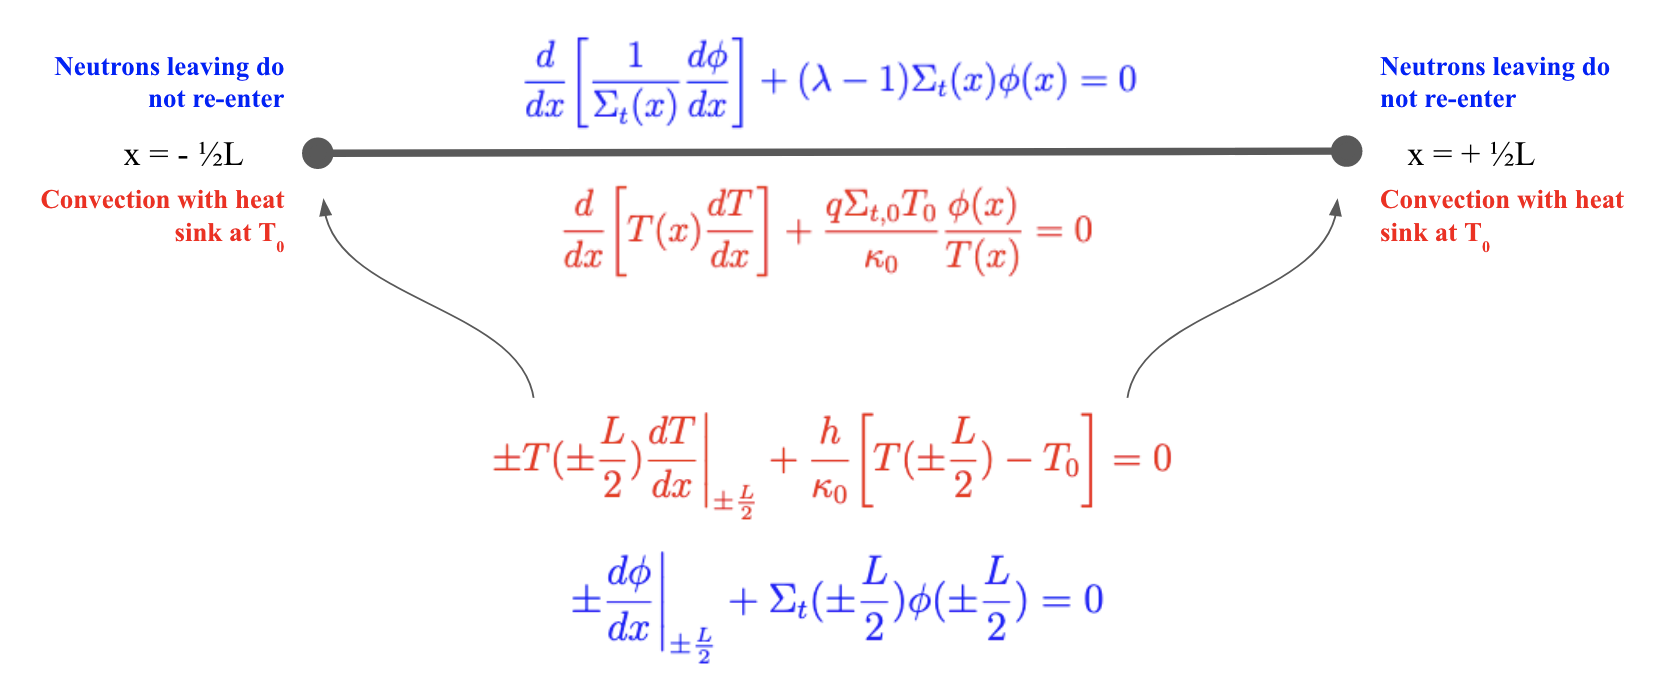
\includegraphics[width=0.65\linewidth]{figures/1D_Benchmark_Diagram.png}
    \caption{This diagram summarizes the domain, \glspl{ode}, and boundary conditions for the slab.}
    \label{fig:slab_diagram}
\end{figure}

This benchmark uses a one-group assumption for the neutron cross-sections. As neutrons transport, heat from fission events deposit
volumetric power in the slab, causing thermal expansion and affecting the temperature distribution; thermal expansion is restricted
to only the $x$-direction. This slab elongation feeds back neutronics and heat conduction by influencing the domain length and
material density. The slab has convective boundary conditions at the endpoints $x=\pm \frac{L}{2}$ with the heat sink temperature
$T_{0}$. The Doppler-broadened total, microscopic cross-section follows an inverse-root temperature relationship,
\begin{equation}
    \sigma_{t}(T) = \sigma_{t,0}\sqrt{\frac{T_{0}}{T(x)}}
\end{equation}
Due to thermal expansion, the slab density varies as
\begin{equation} \label{sec:intro:density}
    \rho(x) =  \rho_{0} \sqrt{\frac{T_{0}}{T(x)}},
\end{equation}
This gives a Doppler-broadened, macroscopic, total cross-section that accounts for changes in density due to temperature as
\begin{equation} \label{sec:intro:doppler}
    \Sigma_{t}(x) = \frac{\rho_{0}\sigma_{t,0} N_{A}}{A} \frac{T_{0}}{T(x)} = \Sigma_{t,0}\frac{T_{0}}{T(x)} ,
\end{equation}
where $ \sigma_{t,0}$ is the total, microscopic cross-section at $T_{0}$, $N_{A}$ is Avogadro's number, and $A$ is the mass number
of the medium. The conduction equation governs heat flow in the slab and can be described in terms of the thermal conductivity
$\kappa(T)$, the energy released per fission $q$, the total, macroscopic cross-section $\Sigma_{t}$, and the neutron flux $\phi$.
\begin{equation}
     \frac{d}{dx}\bigg[\kappa(T(x))\frac{dT(x)}{dx}\bigg] + q \Sigma_{t}(x)\phi(x) = 0.
\end{equation}
The main assumption used to craft the analytical solution is that $T(x)=f\phi(x)$. This assumption is guaranteed by manipulating
the \glspl{ode}, inserting the cross-section temperature dependence, and matching coefficients so that the two \glspl{ode}
are of the same solution type. The matching of coefficients imposes two constraints that give equations for the total, microscopic
cross-section $\sigma_{t,0}$ and the heat transfer coefficient $h$, in terms of the slab parameters. These are two key input
parameters required for the simulation. For full details on the analytical solution's derivation, see \cite{analytical_benchmark}.

\section{COMPUTATIONAL MODEL}
\label{sec:model}
This section describes the OpenMC and \gls{moose} computational models, followed by the convergence criteria used for coupling.
Note that Cardinal currently does not yet support moving geometries in OpenMC. Instead of using thermo-mechanics for thermal
expansion, the simulation uses the formula for equilibrium length $L$ from \cite{analytical_benchmark} that accounts for all
three physics effects. The change in density due to temperature is accounted for in this simulation by using the total, macroscopic
cross-section\ --\ which absorbs density to become a $\frac{1}{T}$ dependence\ --\ from (\ref{sec:intro:doppler}), as was
mentioned in Section \ref{sec:benchmark}.

\subsection{OpenMC Model}
\label{sec:model:OpenMC}
The geometry used in OpenMC must be finite, despite the benchmark being infinite in the $y$ and $z$ directions. In general,
reflective boundary conditions can be used to simulate infinite dimensions. Thus, this benchmark can be represented with
vacuum boundary conditions at $x=\pm \frac{L}{2}$ and reflective boundary conditions at the $y$ and $z$ boundaries. Note that
particles only move in the $\pm x$ direction, so no $y$ or $z$ boundaries are crossed, but with non-$S_{2}$ scattering, the
reflective boundaries would come into play. In addition to being finite for the model, the $y$ and $z$ dimensions need to be
set to $1$ cm in order for Equation (19) from the benchmark to uphold its one dimensional power integral, i.e. that integration in
$y$ and $z$ is implied to contribute a factor of 1. \cite{analytical_benchmark} Fig. \ref{fig:slab_diagram} shows a diagram
of the $1D$ geometry, governing equations, and boundary conditions for the different physics.

The benchmark's one-group assumption was satisfied using OpenMC's multigroup mode. Since the benchmark uses a fictitious material
with a known function for the temperature dependence, the simulation took advantage of OpenMC's capability for user-defined
cross-sections via the \texttt{XSdata} class. The cross-section for each reaction was specified for 50 evenly spaced temperatures
between 308 K and 358 K and was exported to a library that OpenMC used to determine the appropriate cross-section in each region
as temperature changed via input from Cardinal from iteration to iteration.

The OpenMC model required slight source code modifications to accommodate $S_2$-like transport. In typical OpenMC simulations,
the physics of each reaction describes the scattering dynamics. The Monte Carlo algorithm is agnostic to the direction
particles move, but it is not typically constrained to a discrete directional distribution. However, when modeling this
benchmark, any history with a particle moving perpendicular to the $x$-direction would attenuate particles in less
$x$-distance than if particles were constrained to either $\pm x$. To address this, we first use OpenMC's \texttt{PolarAzimuthal}
distribution to restrict the birth direction of particles to the $\pm x$ direction. We then also modified OpenMC in a
patched branch to mimic $S_{2}$ transport in two ways. First, when determining the angular cosine of scattering events,
$\mu$, particles either continue forward ($\mu=1$) or are back-scattered ($\mu=-1$) with equal probability, as opposed to
sampling the reaction physics for $\mu$. Second, since the simulation uses $k$-eigenvalue mode, neutrons born in subsequent
generations of the simulation also need to have their angular birth distributions restricted to $\pm x$.

The k-eigenvalue simulation used 50,000 particles per batch, with 50 inactive batches and 50 active batches for every case. A few
tallies were used in order to compare to the analytical solution: a flux cell tally, a kappa-fission rate cell and global tally,
and the eigenvalue $k_{eff}$. Though flux and the eigenvalue are the only quantities to compare with the benchmark, these other
tallies are needed in order to compute a source strength. OpenMC reports flux, denote it $\hat{\phi}$, in units of $\frac{n-cm}{sp}$,
but typical flux, denote it $\phi$, has units of $\frac{n}{cm^2-s}$. In fixed source modes, the source strength is typically known,
but in eigenvalue mode, it must be computed, as it depends on the physical source and fission source. The following was used to
compute the source strength
\begin{equation} \label{eq:source_strength}
   ss = \frac{P}{\kappa V_{voxel}} \QTHUS \phi = \frac{P}{\kappa V_{voxel} }\hat{\phi},
\end{equation}
where $P=1e22 \frac{ev}{s}$ is the slab integrated power from the benchmark, $\kappa$ is the tallied kappa-fission rate across the slab,
and $V_{voxel}$ is the volume of a voxel in the mesh. The same source strength could be used to convert the kappa-fission tally from
OpenMC, which has units of $\frac{ev}{sp}$, to more physically meaningful units of $\frac{ev}{cm^3-s}$.

\subsection{MOOSE Heat Conduction Model}
The \gls{moose} \gls{hcm} is used to solve for the temperature distribution within the slab. It solves the conduction equation using the
\gls{fem} available in \gls{moose}:
\begin{equation}\label{eq:conduction}
    - \nabla \cdot (k_{s}(\mathbf{r},T_{s}) \nabla T_{s}(\mathbf{r})) = \dot{q}_{s},
\end{equation}
where $k_{s}$ is the thermal conductivity in the solid and $\dot{q}_{s}$ is the heat source, in this case from fission. It uses a
\texttt{HeatConductionMaterial} to specify that the thermal conductivity obeys the benchmark's temperature dependence $\kappa(T)=\kappa_{0}T$.
The boundary conditions used by \gls{moose} match temperature boundary condition in red shown in Fig (\ref{fig:slab_diagram}). The
\gls{hcm} is coupled to OpenMC by receiving the heat source in each element from the kappa-fission tally. During each constituent
iteration, it recomputes the temperature distribution from the heat source and boundary conditions, and then sends the temperatures
back to OpenMC for the next transport solve.

\subsection{Convergence Criteria}
The \gls{hcm} uses iterative methods to compute temperature. It uses a combination of linear and non-linear iterations to update the
solution, stopping once both of the convergence criteria are met. This study used convergence criteria of $10^{-7}$ for absolute tolerance
and $10^{-9}$ for relative tolerance.  The following petsc options were included:
\begin{lstlisting}
    petsc_options_iname=`-pc_type -pc_hypre_type'
    petsc_options_value=`hypre boomeramg'
\end{lstlisting}
Monte Carlo is not an iterative method, so convergence is achieved by using an
appropriate number of batches and histories per batch. The configurations used here were mentioned in Section \ref{sec:model:OpenMC}.

In terms of converging global iterations across all single physics, each mesh cases used 200 Picard Iterations. To assist with
convergence of Monte Carlo quantities, Robbins-Monro relaxation was applied to the flux and kappa-fission tallies. This updates the
quantities of interest for the $n+1$th iteration as an average over the newest solution and the $n$ previous iterations. \cite{omccap}
So the flux at Picard Iteration $n+1$ would be given by
\begin{equation}\label{eq:Robbins-Monro}
    \phi_{n+1} = \frac{1}{n+1} \sum_{i=0}^{n} \phi_{i},
\end{equation}
where $\phi_{i}$ is the flux output from the $i$th Monte Carlo solve. In order to assess the convergence of each physics, plots of
error versus mesh element size were used and will be shown in Section \ref{sec:results}.

\section{RESULTS}\label{sec:results}
The results to compare with the benchmark are the temperature distribution, flux distribution, and eigenvalue. The benchmark provides
analytical solutions for all of these quantities. An example temperature distribution is shown in the figure below for the 50 mesh element case.
\begin{figure}[H]
    \centering
    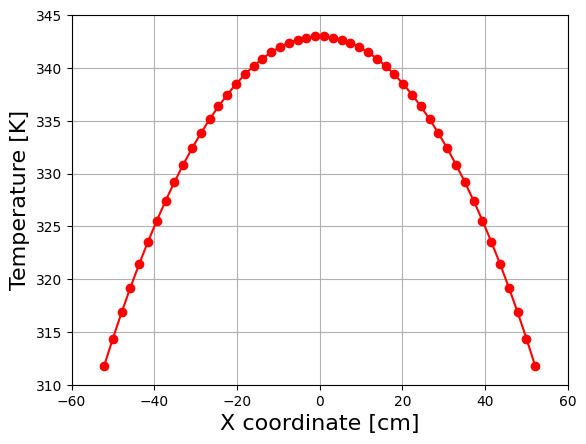
\includegraphics[width=0.55\linewidth]{figures/temp_50.png}
    \caption{This plot shows the computed temperature for 50 mesh elements.}
    \label{fig:temp50}
\end{figure}
In order to assess the accuracy of the temperature solution and verify that refining the mesh increases the accuracy, the analytical solution
was used to compute an $L_{2}$ error norm for temperature. The error computed, $\epsilon_{T}$, is given by
\begin{equation}
    \epsilon_{T} = \frac{|| T_{a} - T_{x} ||_{2}}{|| T_{a} ||_{2}},
\end{equation}
where $T_{a}$ is the analytical solution evaluated at the x-centroid of the mesh element and $T_{x}$ is the temperature computed for that
voxel from the multiphysics simulation. The figure below shows how the temperature error relates to the number of mesh elements
\begin{figure}[H]
    \centering
    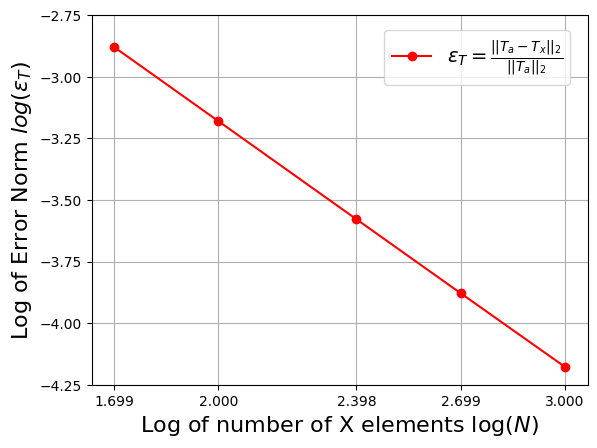
\includegraphics[width=0.45\linewidth]{figures/temp_error_norms.png}
    \caption{This plot shows log of the number of mesh elements vs the log of the $L_{2}$ error norm for the computed vs analytical temperature.}
    \label{fig:temp_error_study}
\end{figure}
Linear convergence is achieved, as the slope of the line on the $\log(N)$ vs $\log(\epsilon_{T})$ plot is $-0.99924828$. The same convergence test
was used on the flux solution as well with the flux error norm, $\epsilon_{\phi}$, defined as
\begin{equation}
    \epsilon_{\phi} =  \frac{|| \phi_{a} - \phi_{x} ||_{2}}{|| \phi_{a} ||_{2}}.
\end{equation}
The figure below shows how the flux error relates to the number of mesh elements
\begin{figure}[H]
    \centering
    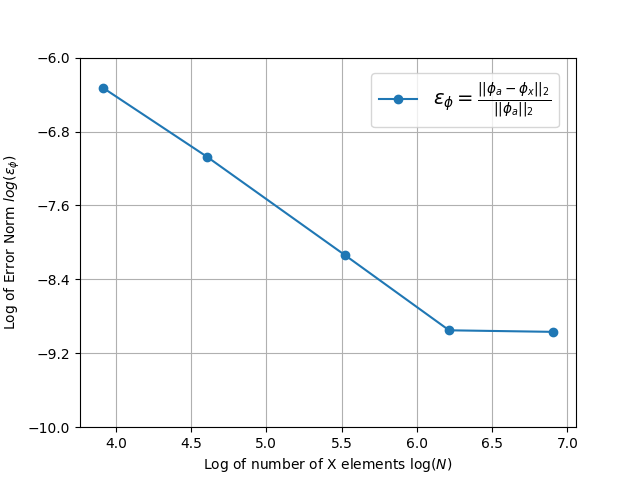
\includegraphics[width=0.45\linewidth]{figures/flux_error_norms.png}
    \caption{This plot shows log of the number of mesh elements vs the log of the $L_{2}$ error norm for the computed vs analytical flux.}
    \label{fig:flux_error_study}
\end{figure}
[CONVERGENCE] , as the slope of the line on the $\log(N)$ vs $\log(\epsilon_{\phi})$ plot is \textbf{TODO SLIGHT PROBLEM W FLUX LAST BIN CONVERGENCE}.
Another measure of comparison is the \gls{ce} for each mesh size. The ideal would be exact equality, or a ratio of $1$. The temperature
and flux \glspl{ce} are shown in the figure below.
\begin{figure}[H]
    \centering
    \begin{minipage}[b]{0.48\linewidth}
        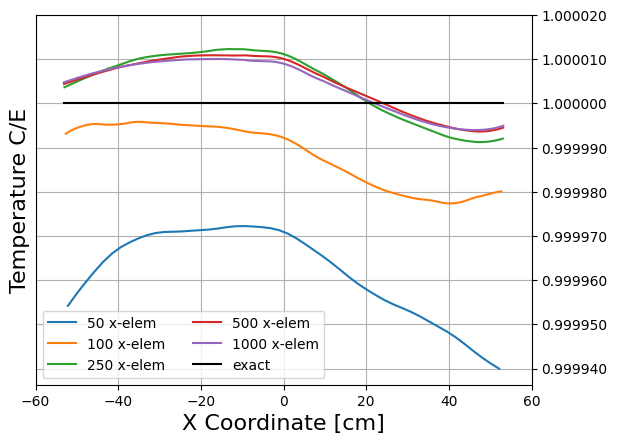
\includegraphics[width=\linewidth]{figures/temp_num_to_analy_ratios.png}
    \end{minipage}
    \begin{minipage}[b]{0.48\linewidth}
        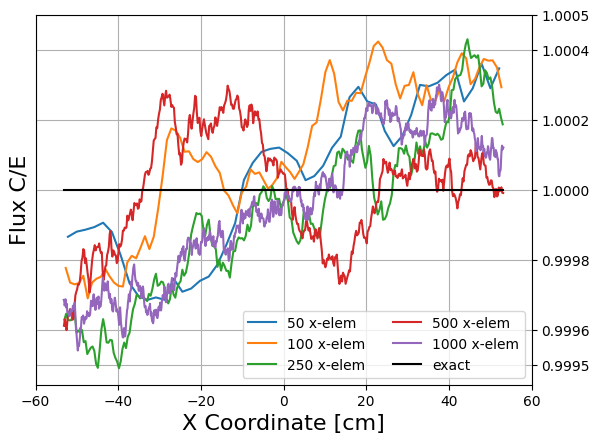
\includegraphics[width=\linewidth]{figures/flux_num_to_analy_ratios.png}
    \end{minipage}
\end{figure}
Lastly, the eigenvalue for each mesh is reported in the table below.
\begin{table}[H]
    \centering
    \caption{Eigenvalue with uncertainty for each mesh size. TODO update and get the newest ones}
    \begin{tabular}{c|c|c}
        \textbf{mesh elements} & $k_{eff}$ & pcm diff \\
        \hline
        50 & 0.29555 $\pm$ 0.00009 & 9 \\
        100 & 0.29551 $\pm$ 0.00011 & 6 \\
        250 & 0.29585  $\pm$ 0.00012 &  -28 \\
        500 & 0.29574 $\pm$ 0.00013 & -17 \\
        1000 & 0.29551 $\pm$ 0.00013 & 6
    \end{tabular}
    \label{tab:data}
\end{table}

\section{CONCLUSIONS}\label{sec:conclusions}

Overall, the numerical results show strong agreement with the analytical solutions. The convergence is first order for the temperature
and \textbf{flux}.The stochastic nature of the Monte Carlo algorithm is likely a factor for the convergence of the flux. Since zeroth
order shape functions are used in the \gls{fem}, the first order temperature spatial convergence is to be expected. \cite{moose-convergence}
The \gls{ce} plots also show expected behavior. As the mesh fineness increases, the computed to expected ratio gets closer and closer to
the ideal $y=1$. The eigenvalue agrees very well for all cases and appears to be independent of the mesh size.

While code to code benchmarking is common in for nuclear \gls{ms}, agreement with analytical benchmarks greatly increases the confidence
in Cardinal's multiphysics coupling. Though typical industry-grade simulations would not run $S_{2}$ transport, this modification allows
Cardinal to show it can match against theoretical expectations.

\textit{future work to mention?}

\section*{NOMENCLATURE}

% TODO fix glossary
\printglossary[title={Nomenclature}, nonumberlist, nopostdot]

\section*{ACKNOWLEDGEMENTS}
The authors would like to thank the OpenMC and MOOSE development teams for their guidance in model setup and assistance
with software. We also want to thank Dr. Griesheimer and Dr. Kooreman for their modeling advice and knowledge about the
analytical benchmark.

\setlength{\baselineskip}{12pt}
\bibliographystyle{mc2023}
\bibliography{mc2023}
\setlength{\baselineskip}{12pt}


\end{document}
